\documentclass[ngerman,hyperref={pdfpagelabels=false}]{beamer}

% -----------------------------------------------------------------------------

\graphicspath{{images/}}

% -----------------------------------------------------------------------------

\usetheme{KIT}

\setbeamercovered{transparent}
%\setbeamertemplate{enumerate items}[ball]

\newenvironment<>{KITtestblock}[2][]
{\begin{KITcolblock}<#1>{#2}{KITblack15}{KITblack50}}
{\end{KITcolblock}}

\usepackage[ngerman,english]{babel}
\usepackage[utf8]{inputenc}
\usepackage[TS1,T1]{fontenc}
\usepackage{array}
\usepackage{multicol}
\usepackage[absolute,overlay]{textpos}
\usepackage{beamerKITdefs}
\usepackage{amsfonts}


\pdfpageattr {/Group << /S /Transparency /I true /CS /DeviceRGB>>}	%required to prevent color shifting withd transparent images


\title{A Linear-Time Algorithm For Finding Tree-Decompositions Of Small Treewidth}
\subtitle{Maximilian F. Göckel -- \textit{uzkns@student.kit.edu}}

\author[Maximilian Göckel]{Maximilian F. Göckel}
\institute{Institut für Theoretische Informatik - Proseminar Algorithmen für NP-schwere Probleme}

\TitleImage[width=\titleimagewd,height=\titleimageht]{titel}

\KITinstitute{Institut f\"ur Theoretische Informatik}
\KITfaculty{Proseminar NP-schwere Probleme}

% -----------------------------------------------------------------------------

\begin{document}
\setlength\textheight{7cm} %required for correct vertical alignment, if [t] is not used as documentclass parameter


% title frame
\begin{frame}
  \maketitle
\end{frame}


\begin{frame}
\frametitle{Motivation}
Viele (NP-schwere) Graphenprobleme sind auf Graphen, bei denen eine Baumzerteilung mit Baumweite max. $k$ ($k$ Konstante) gegeben ist, in Linearzeit lösbar. \\
\ \\
%Zum Beispiel das Hamiltonkreisproblem.
	
\end{frame}


%%treedecomp
%\begin{frame}
%  \frametitle{Tree-decomposition}
%  Jeder Graph kann zu einem Baum umgewandelt ("zerteilt") werden. \\
%  \ \\
%  \begin{itemize}
%  	\item Der Graph ist bereits ein Baum $\Rightarrow$ fertig
%  	\item Der Graph ist kein Baum $\Rightarrow$ Baumzerteilung anwenden
%  \end{itemize}	
%\end{frame}


%Voraussetzungen
\begin{frame}
\frametitle{Tree-decomposition: Definition}
\ \\ 
Eine Baumzerteilung eines Graphen $G=(V,E)$ ist ein Tupel $(X, T)$ wo $T =(I, F)$ ein Baum ist und $X = \{ X_i | i \in I \}$ eine Familie von Teilmengen von $V$ wobei jedes $X_i$ einen Knoten in $T$ darstellt. \\
\ \\
\begin{enumerate}
	\item $\bigcup\limits_{i \in I} X_i = V$
	\item $\forall (v,w) \in E: \exists i \in I: v,w \in X_i$
	\item $\forall w \in X_i, X_j : $ Jedes $X_k$ im Pfad zwischen $X_i, X_j$ enthält $w$
\end{enumerate}
\end{frame}


%Beispiel
\begin{frame}
\frametitle{Tree-decomposition: Beispiel}

\begin{figure}[htbp] 
	\centering
	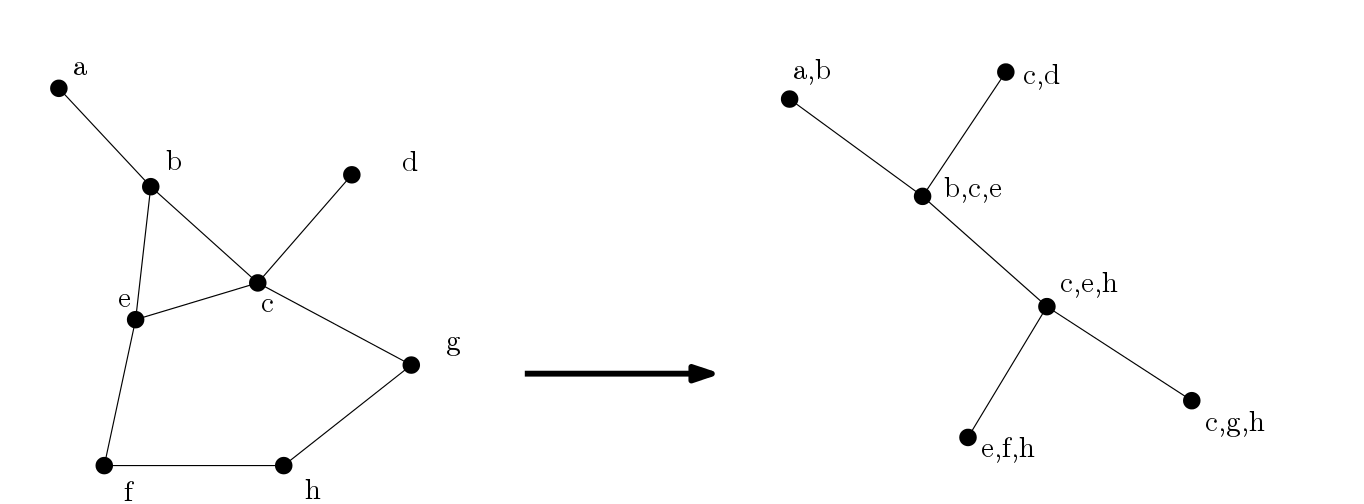
\includegraphics[width=0.7\textwidth]{tree_2.png}
	\caption{1}
	\label{fig:Bild1}
\end{figure}

\end{frame}


%\begin{frame}
%\frametitle{Tree-decomposition: Beispiel}
%
%\begin{figure}[htbp] 
%	\centering
%	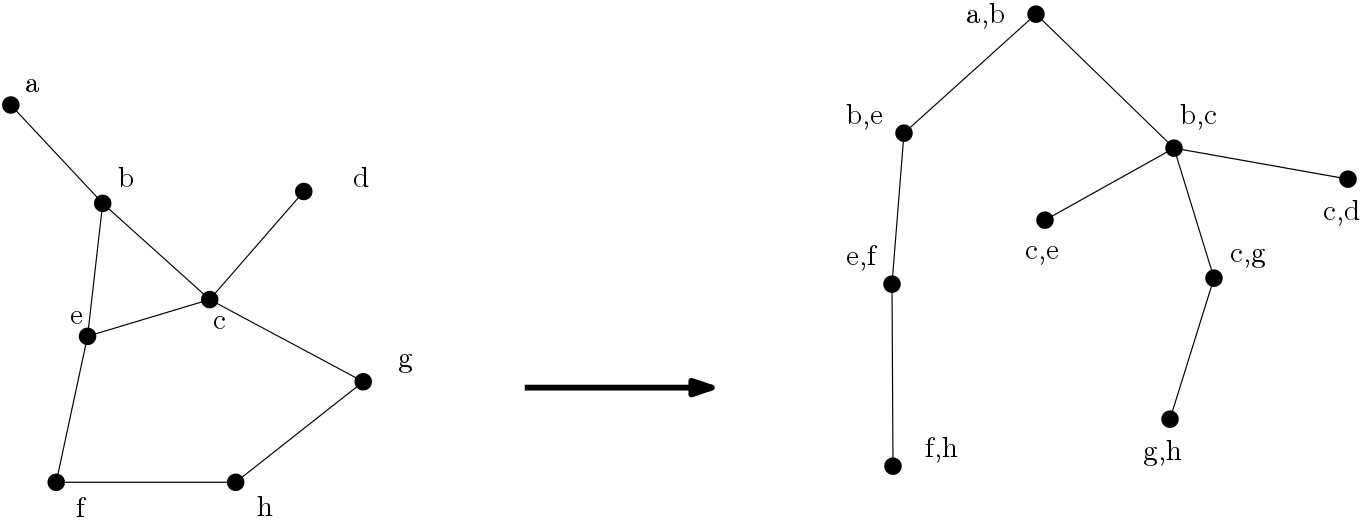
\includegraphics[width=0.7\textwidth]{tree_1.png}
%	\caption{2}
%	\label{fig:Bild1}
%\end{figure}
%
%\end{frame}


%treewidth
\begin{frame}
\frametitle{Treewidth}

Jede Baumzerteilung hat eine "Baumweite" (treewidth). \\

\begin{itemize}
	\item Baumweite einer Zerteilung: ${\max}( {|X_i|}_{i \in I} - 1)$ ("Zerteilungsweite")
	\item Baumweite eines Graphen: Minimale Zerteilungsweite aller Zerteilungen
\end{itemize}

\end{frame}




\begin{frame}
\frametitle{Hauptidee}

Viele NP-schwere Probleme sind in Linearzeit lösbar, wenn die Baumweite des Graphen konstant ist. $\rightarrow$ Kann man die Baumweite (für bel., festes $k \in \mathbb{N}$) in Linearzeit errechnen? \\
\ \\
$\mathrm{Z\kern-.3em\raise-0.5ex\hbox{Z}}$: $\forall k \in \mathbb{N}: \exists$ Linearzeitalgorithmus welcher für $G=(V,E)$ prüft ob die Baumweite max. $k$ ist und eine Zerteilung ausgibt. \\
\ \\
Für $k = 1,2,3,4$ existieren schon Linearzeitalgorithmen
\end{frame}


%Algo
\begin{frame}
\frametitle{Algorithmus}
2 Schritte: \\
\begin{enumerate}
	\item Für gegebenen Graph $G = (V,E)$ und geg. $k \in \mathbb{N}$ eine Zerteilung mit max. Baumweite linear in $k$ finden
	\item Graph-Zugehörigkeit zur Klasse "Graphen mit Baumweite $k$" prüfen
\end{enumerate}
\ \\
\ \\
Problem \textit{"Für einen Graph $G=(V,E)$ und ein $k \in \mathbb{N}$: Ist die Baumweite von $G$ maximal $k$?"} ist NP-Vollständig für bel. $k$ \\
\ \\

\end{frame}
















\end{document}
